\section{Análisis y diseño}

% cFE

\begin{frame}{Core Flight Executive (cFE)}

\begin{figure}
\center
\resizebox{!}{.33\textheight}{\begin{tikzpicture}[
	every node/.style={rectangle,font=\large,align=center,
	                   minimum height=0.66cm,text width=10cm,
	                   on chain,draw=olive!60!black!50},
	start chain=going above, node distance=8pt,
]

\node  [fill=olive!50!black!16] {Hardware};
\node  [fill=olive!50!black!14]  {Operating System (Linux, RTEMS, VxWorks, FreeRTOS)};
\node  [fill=olive!50!black!12] {Operating System Abstraction Layer (OSAL)};
\node  [fill=olive!50!black!10]  {cFE Services (Exec, Event, Bus, Table, Time)};
\node  [fill=olive!50!black!8] {cFS/User		Applications/Libraries};

\end{tikzpicture}}
\caption{Arquitectura sistema CFS}

\end{figure}

cFE es un OBSW desarrollado por NASA, que se caracteriza por:

\begin{itemize}
\item \emph{Framework} de desarrollo y entorno de ejecución.
\item Conjunto de servicios (Software Bus, Time, Events, etc).
\item Análisis de rendimiento en tiempo real.
\item Arquitectura modular.
\end{itemize}

\end{frame}


% Arquitectura global

\begin{frame}{Arquitectura de la misión}

\begin{figure}
\centering
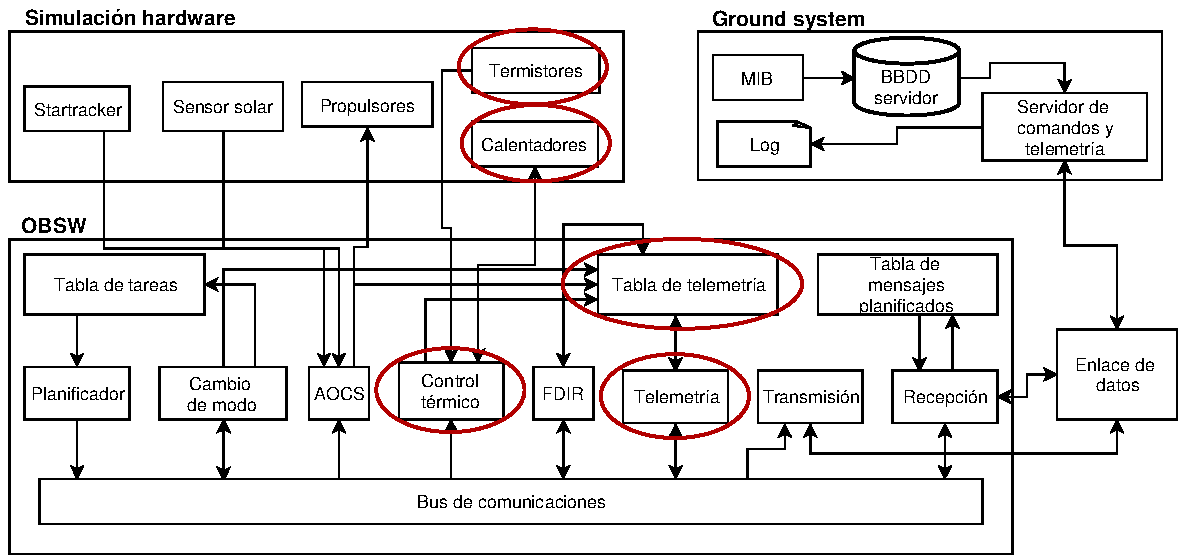
\includegraphics[width=\textwidth]{/arquitecturadelsistema}
\caption{Arquitectura de la misión}
\end{figure}

El sistema se compone de tres subsistemas:  Simulación hardware, OBSW y ground system.

\end{frame}


% Diagrama de componentes

\begin{frame}{Diseño de la solución}

\begin{figure}[h]
\centering
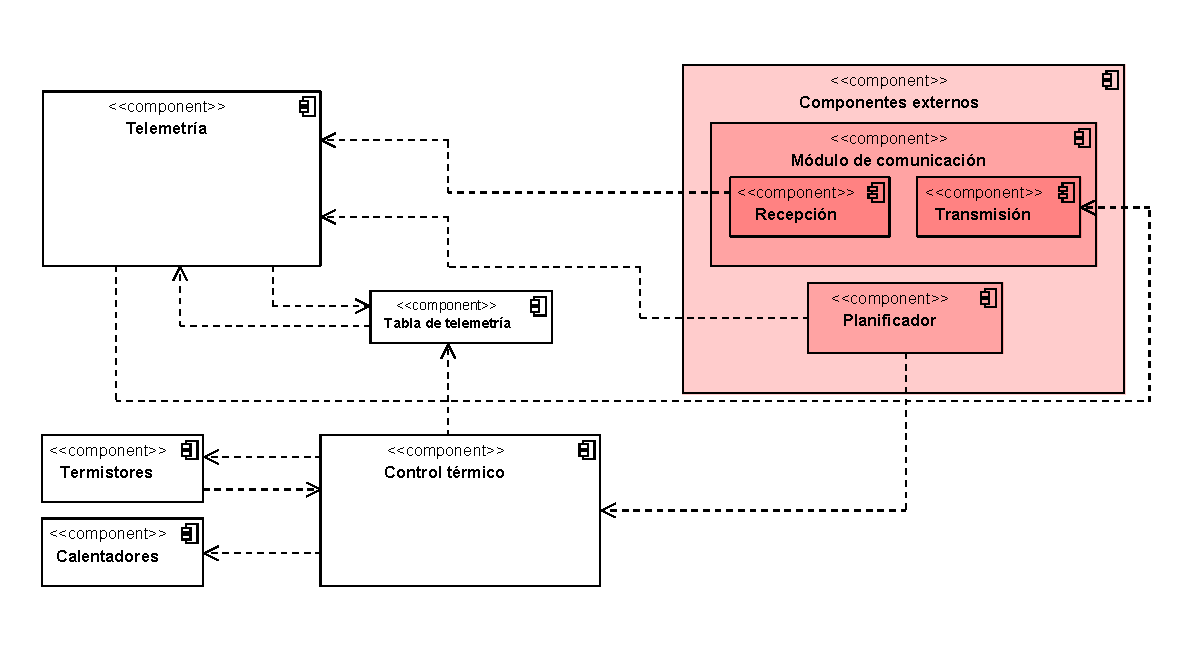
\includegraphics[width=\textwidth]{diagramacomponentes}
\caption{Diagrama de componentes}
\end{figure}

\end{frame}
